% Index-3 pendulum, the classic DAE example (Ascher & Petzold).
%
% AXES ARE AT THE PIVOT, not at the bob. The model is
%
%     xddot = -T x,    yddot = g - T y,    x^2 + y^2 = 1
%
% so (x,y) is the bob's position MEASURED FROM THE PIVOT, and the algebraic
% constraint says it lies at unit distance from the origin. Drawing the axes at
% the bob would put the bob at the origin and make x^2 + y^2 = 1 false.
%
% An earlier version of this figure did exactly that, and was published to the
% website that way. Corrected 2026-08-17 to match the mathematics and the
% Fall 2018 scan, which also places the axes at the pivot.
%
% y is positive DOWNWARD, which is what makes yddot = g - T y correct with
% g > 0. x is positive to the right, so the bob drawn down-and-right has
% x > 0 and y > 0.

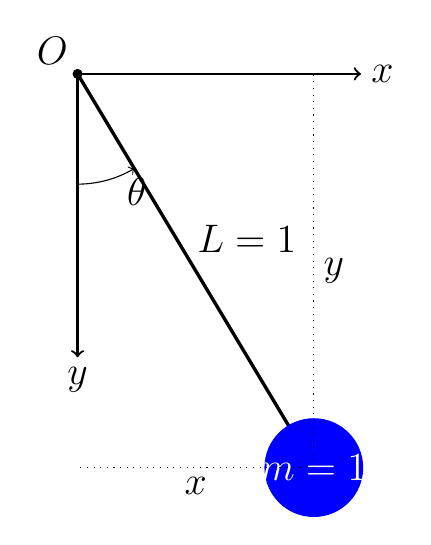
\begin{tikzpicture}

% Pivot: the origin of the coordinate system
\filldraw[black] (-1, 3) circle (1.6pt);
\node[above left] at (-1, 3) {\Large $O$};

% Coordinate axes, rooted AT THE PIVOT
\draw[->, thick] (-1, 3) -- (2.6, 3) node[right] {\Large $x$};
\draw[->, thick] (-1, 3) -- (-1, -0.6) node[below] {\Large $y$};

% Reference vertical, and the angle from it
\draw[dashed] (-1, 3) -- (-1, 0.2);
\draw[->] (-1, 1.6) arc (270:301:1.4);
\node at (-0.25, 1.5) {\Large $\theta$};

% Pendulum arm
\draw[very thick] (-1, 3) -- (2, -2);
\node at (1.15, 0.9) {\Large $L = 1$};

% Bob
\filldraw[blue] (2, -2) circle (0.62cm);
\node[white] at (2, -2) {\Large $m = 1$};

% Components of the bob position, measured from the pivot
\draw[dotted] (2, -2) -- (2, 3) node[midway, right] {\Large $y$};
\draw[dotted] (2, -2) -- (-1, -2) node[midway, below] {\Large $x$};

\end{tikzpicture}
